\documentclass[aspectratio=1610,14pt,t]{beamer}

% Colors
\usepackage{color}
\definecolor{mainorange}{HTML}{EC811B}
\definecolor{lightgrey}{HTML}{888888}
\definecolor{almostwhite}{HTML}{FEFEFE}

% Syntax highlighting
\usepackage{minted}
\usepackage{alltt}
\newcommand\hi[1]{{\color{mainorange} \textbf{#1}}}

\usepackage{wasysym}

% Custom unicode symbols
\usepackage{newunicodechar}
\newcommand\Warning{%
 \makebox[1.4em][c]{%
 \makebox[0pt][c]{\raisebox{.1em}{\small!}}%
 \makebox[0pt][c]{\color{red}\Large$\bigtriangleup$}}}%

\newunicodechar{⚠}{\Warning}

% Theme
\usetheme[%
  subsectionpage=progressbar,
  numbering=fraction,
  progressbar=foot,
]{metropolis}

% Customization
\usepackage{pagecolor}
\setbeamertemplate{section in toc}[sections numbered]
\setbeamerfont{title}{size=\fontsize{30}{30}}
\setbeamerfont{block title}{size=\large}
\newcommand\sep{\textcolor{lightgrey}{\rule{\linewidth}{0.05mm}}}

% Positioning
% https://tex.stackexchange.com/a/34929/13059
\def\Put(#1,#2)#3{\leavevmode\makebox(0,0){\put(#1,#2){#3}}}

% Meta
\title{Embedded Rust}
\date{2018-12-11}
\author{Raphael Nestler (@rnestler)}
\institute{Rust Zürichsee Meetup}

\begin{document}

\pgfdeclareimage[width=\paperwidth]{bg}{background-dark.pdf}
\pagecolor{almostwhite}  % Prevent speakerdeck from optimizing away the bg color
\usebackgroundtemplate{\pgfuseimage{bg}}
\maketitle

% ----------------------------------------------------------------- %

\begin{frame}[c]{println!("{:?}", Self)}
  Hi! I'm Raphael (@rnestler).

  \pause I live in Rapperswil

  \pause I work at Sensirion ({\small \url{https://sensirion.com}}).

  \pause I'm a founding member of Coredump\\hackerspace ({\small \url{https://coredump.ch}}).
\end{frame}

% ----------------------------------------------------------------- %

\begin{frame}[plain,noframenumbering]
  \frametitle{Outline}
  \setcounter{tocdepth}{1}
  \tableofcontents
\end{frame}

% ----------------------------------------------------------------- %

\pgfdeclareimage[width=\paperwidth]{bg}{background-light.pdf}
\usebackgroundtemplate{\pgfuseimage{bg}}

\section{Embedded Programming}

\begin{frame}[c]{What is an \emph{Embedded System}?}
  \begin{quote}
    A combination of computer hardware and software, and perhaps
    additional mechanical or other parts, designed to perform a dedicated
    function.
  \end{quote}
  Michael Barr. ``Embedded Systems Glossary''\footnote{\tiny\url{https://barrgroup.com/Embedded-Systems/Glossary-E\#embedded\_system}}
\end{frame}

\begin{frame}[c]{What is embedded programming?}
  \begin{itemize}
    \item Dedicated, not general purpose, µC system
    \item<1-> Baremetal
    \item<1-> Low-Level
    \item<2-> For this talk: Bare metal on Cortex-M MCUs
  \end{itemize}
\end{frame}

\begin{frame}[c]{Why do they say it's hard?}
  \begin{itemize}
    \item Harsh environment (No OS which protects you)
    \item Resource constrained (Remember dedicated?)
    \item Non-standard, Non-OSS toolchain
    \item Hard realtime requirements
    \item \ldots
  \end{itemize}
\end{frame}

\begin{frame}[c]{Why could Rust be awesome for it?}
  \begin{itemize}
    \item Zero cost abstractions!
    \item Provides safety at compiler level, not OS
    \item Expressive type system to encode constraints
  \end{itemize}
\end{frame}

\section{State of Embedded in 2018}
\begin{frame}[c]{You can use stable!}
  \begin{itemize}
    \item Previously we needed nightly for \texttt{no\_std} binaries
    \item Rust 1.6 \texttt{no\_std / libcore} gets
      introduced\footnote{\url{https://blog.rust-lang.org/2016/01/21/Rust-1.6.html}}
    \item Rust 1.27 cortex-m embedded libraries possible on stable\footnote{\url{https://twitter.com/japaricious/status/995633889858277376}}
    \item Rust 1.30 embedded binaries possible on
      stable\footnote{\url{https://blog.rust-lang.org/2018/10/25/Rust-1.30.0.html}}
    \item I recommend to use Rust 1.31 2018 edition (Released recently)
  \end{itemize}
\end{frame}

\begin{frame}[c]{You can use stable!\footnote{\url{https://hacks.mozilla.org/2018/12/rust-2018-is-here/}}}
  \centering
  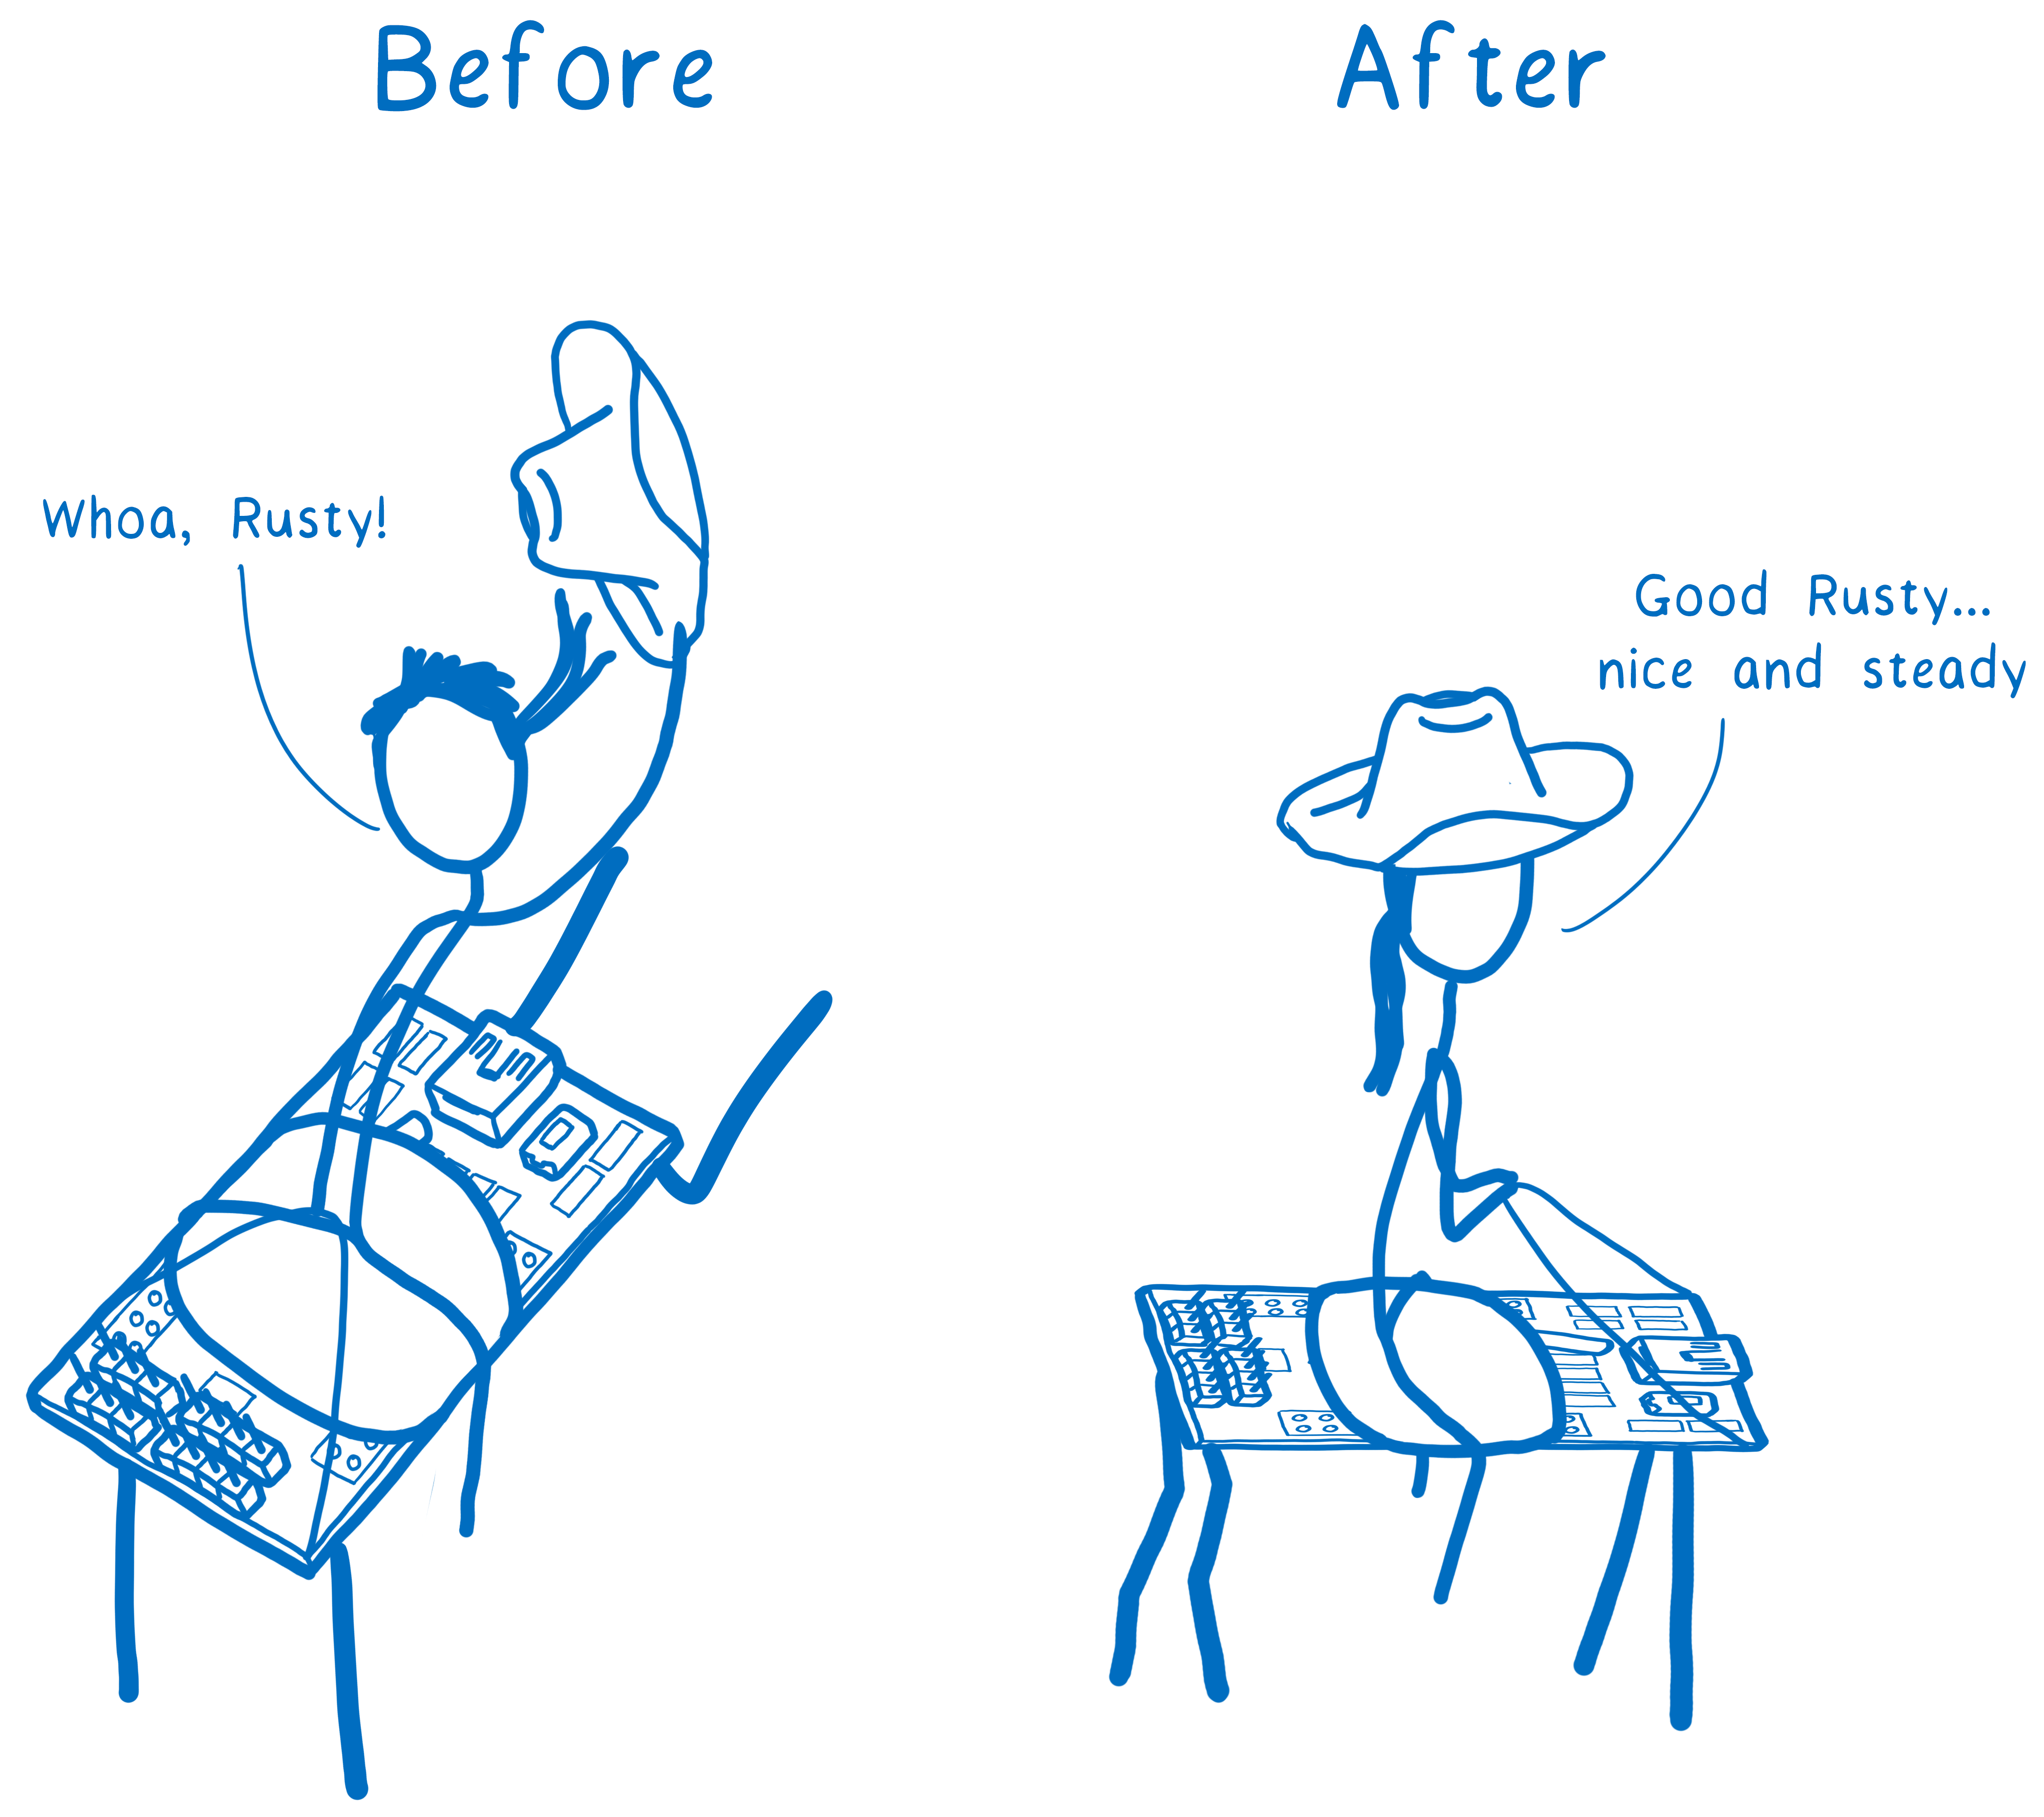
\includegraphics[width=.6\textwidth]{img/embedded-is-stable.png}
\end{frame}

\begin{frame}[c]{No more lib core cross compiling}
  \begin{itemize}
    \item Previously we needed to use
      xargo\footnote{\url{https://github.com/japaric/xargo}} to cross compile
      lib core
    \item Now Cortex-M targets are supported by rustup / cargo
      (thumbvxx-none-eabi)
  \end{itemize}
\end{frame}

\begin{frame}[c]{Collaborative Effort}
  \begin{itemize}
    \item Rust Embedded Working Group
    \item Started in the beginning of 2018\footnote{\url{https://rust-embedded.github.io/blog/2018-03-15-newsletter-1/}}
    \item Works on
      \begin{itemize}
        \item Documentation (Blog posts, The Embedded Rust Book, \ldots)
        \item Tooling (LLVM, rustc, \ldots)
        \item Standartization in the ecosystem (embedded-hal, \ldots)
      \end{itemize}
  \end{itemize}
\end{frame}

\begin{frame}[c]{More Resources}
  \begin{itemize}
    \item The Rust Embedded Book\footnote{\url{https://docs.rust-embedded.org/book/}}
    \item The Embedded Bookshelf\footnote{\url{https://docs.rust-embedded.org/}}
    \item The Discovery book\footnote{\url{https://docs.rust-embedded.org/discovery/index.html}}
  \end{itemize}
\end{frame}

\section{Getting started – STM32F3 Discovery}

\begin{frame}[c]{Prerequisites}
  \begin{itemize}
    \item \Square Target support by compiler
    \item \Square Libcore compiled for the target
    \item \Square A Peripheral Access crate (PAC)
    \item \Square Runtime to setup micro controller
  \end{itemize}
\end{frame}

\begin{frame}[c]{Prerequisites}
  \begin{itemize}
    \item \CheckedBox Target support by compiler
    \item \CheckedBox Libcore compiled for the target
    \item \Square A Peripheral Access crate (PAC)
    \item \Square Runtime to setup micro controller
  \end{itemize}
\end{frame}

\begin{frame}[c]{svd2rust}
  \begin{itemize}
    \item Every Cortex-M μC vendor must provide an SVD (System View
      Descriptions) file
    \item SVD is an XML standard to describe peripheral registers
    \item svd2rust\footnote{\url{https://github.com/japaric/svd2rust}}:
      Generate Rust register maps (structs) from SVD files
    \item Done for our μC family\footnote{\url{https://github.com/japaric/stm32f30x}}
  \end{itemize}
\end{frame}

\begin{frame}[c]{Prerequisites}
  \begin{itemize}
    \item \CheckedBox Target support by compiler
    \item \CheckedBox Libcore compiled for the target
    \item \CheckedBox A Peripheral Access crate (PAC)
    \item \Square Runtime to setup micro controller
  \end{itemize}
\end{frame}

\begin{frame}[c]{cortex-m, cortex-m-rt}
  \begin{itemize}
    \item The cortex-m\footnote{\url{https://github.com/rust-embedded/cortex-m}} crate gives access to common low level features of all Cortex-M devices.
    \item The cortex-m-rt\footnote{\url{https://github.com/rust-embedded/cortex-m-rt}} implements a runtime for Cortex-M μCs
  \end{itemize}
\end{frame}

\begin{frame}[c]{Prerequisites}
  \begin{itemize}
    \item \CheckedBox Target support by compiler
    \item \CheckedBox Libcore compiled for the target
    \item \CheckedBox A device crate (access to the target peripherals)
    \item \CheckedBox Runtime to setup micro controller
  \end{itemize}
\end{frame}

\begin{frame}[c,fragile]{Install Toolchain\footnote{\url{https://rust-embedded.github.io/book/intro/tooling.html}}}
  \begin{minted}[fontsize=\footnotesize]{bash}
  $ rustup override set 1.31.0
  $ rustc --version
  rustc 1.31.0 (abe02cefd 2018-12-04)
  $ rustup target add thumbv7em-none-eabihf
  $ rustup component add llvm-tools-preview
  $ cargo install cargo-generate
  $ cargo install cargo-binutils
  \end{minted}
\end{frame}

\begin{frame}[c,fragile]{cortex-m-quickstart}
  \begin{minted}[fontsize=\footnotesize,breaklines]{bash}
  $ cargo generate --git https://github.com/rust-embedded/cortex-m-quickstart --name hello-discovery
  $ cd hello-discovery
  $ vim .cargo/config
  # Cortex-M4 -> thumbv7em
  # (https://en.wikipedia.org/wiki/ARM_Cortex-M)
  +[build]
  +target = "thumbv7em-none-eabihf"
  $ vim memory.x # from datasheet
  CCRAM : ORIGIN = 0x10000000, LENGTH = 8K
  FLASH : ORIGIN = 0x08000000, LENGTH = 256K
  RAM : ORIGIN = 0x20000000, LENGTH = 40K
  \end{minted}
\end{frame}

\begin{frame}[c,fragile]{Building / Running}
  \begin{minted}[fontsize=\footnotesize,breaklines]{bash}
  $ cargo build --example hello
  # separate terminal
  $ openocd openocd.cfg
  # Optional if the above fails
  $ lsusb|grep ST-LINK
  Bus 001 Device 004: ID 0483:374b STMicroelectronics ST-LINK/V2.1
  $ sudo chgrp input /dev/bus/usb/001/004
  $ arm-none-eabi-gdb -x openocd.gdb -q target/thumbv7em-none-eabihf/debug/examples/hello
  ...
  (gdb) continue
  # Other terminal
  Hello, world!
  semihosting: *** application exited ***
  \end{minted}
\end{frame}

\begin{frame}[c]{Semihosting? Sorcery!}
  \centering
  
\includegraphics[width=.7\textwidth]{img/what-sorcery-is-this.jpg}
\end{frame}

\begin{frame}[c,fragile]{Hello World using semi hosting\footnote{\url{https://rust-embedded.github.io/book/start/semihosting.html}}}
  Kind of ``system calls'' into debugger
  \begin{itemize}
    \item Breakpoint instruction with a special tag. $\rightarrow$ Debugger
      gets notified.
    \item Two registers indicate which procedure call and points to a structure
      with arguments.
    \item The debugger reads the memory to retrieve the arguments and passes
      these on to the host's procedure.
    \item The target's CPU is unhalted and execution continues.
  \end{itemize}
  \begin{minted}[fontsize=\footnotesize]{bash}
  \end{minted}
\end{frame}

\begin{frame}[c,fragile]{Hello World explained}
  \begin{minted}[fontsize=\small]{rust}
  ...
  use cortex_m_semihosting::hprintln;
  ...
  #[entry]
  fn main() -> ! {
    hprintln!("Hello, world!").unwrap();
    loop {}
  }
  \end{minted}
\end{frame}

\section{RTFM}
\subsection{Real Time For the Masses}

\begin{frame}[c]{What is RTFM?}
  \begin{quote}
    Framework based on the RTFM language created by the Embedded Systems group
    at Luleå University of Technology, led by Prof. Per Lindgren.
  \end{quote}
  The cortex-m-rtfm book \footnote{\url{https://japaric.github.io/cortex-m-rtfm/book/preface.html}}
\end{frame}

\begin{frame}[c]{Features of RTFM}
  \begin{itemize}
      \item Tasks Triggered asynchronously or by the application
      \item Message Passing between tasks
      \item Timer queue (schedule in the future, periodic)
      \item Priorization of tasks
      \item Efficient and data race free memory sharing
      \item \strong{Deadlock free execution} guaranteed at compile time.
      \item Uses the hardware for scheduling
  \end{itemize}
\end{frame}

\begin{frame}[c,fragile]{Minimal Example}
  \small{Follow along: \url{https://github.com/rnestler/hello-rtfm-rs/tree/minimal-example}}
  \begin{minted}[fontsize=\tiny]{rust}
#![no_std]
#![no_main]
extern crate panic_semihosting; // logs messages to the host stderr; requires a debugger

use cortex_m_semihosting::hprintln;
use rtfm::app;

#[app(device = stm32f30x)]
const APP: () = {
    #[init]
    fn init() {
        hprintln!("init").unwrap();
    }
    #[idle]
    fn idle() -> ! {
        hprintln!("idle").unwrap();
        loop {}
    }
};
  \end{minted}
\end{frame}

\begin{frame}[c,fragile]{Minimal Example}
  \small{Follow along: \url{https://github.com/rnestler/hello-rtfm-rs/tree/minimal-example}}

  Output:
  \begin{minted}[fontsize=\small]{rust}
    init
    idle
  \end{minted}
\end{frame}

\begin{frame}[c,fragile]{Switching contexts}
  \small{Follow along: \url{https://github.com/rnestler/hello-rtfm-rs/tree/first-demo}}
  \begin{minted}[fontsize=\tiny]{rust}
#[app(device = stm32f30x)]
const APP: () = {
    #[init]
    fn init() {
        rtfm::pend(Interrupt::SPI1);
        hprintln!("init").unwrap();
    }
    #[idle]
    fn idle() -> ! {
        hprintln!("idle").unwrap();
        rtfm::pend(Interrupt::SPI1);
        hprintln!("idle 2").unwrap();
        loop {}
    }
    #[interrupt]
    fn SPI1() {
        static mut TIMES: u32 = 0;
        *TIMES += 1; // Safe access to local `static mut` variable
        hprintln!("SPI1 called {} time{}", *TIMES, if *TIMES > 1 { "s" } else { "" }).unwrap();
    }
};
  \end{minted}
\end{frame}


\begin{frame}[c,fragile]{Switching contexts}
  \small{Follow along: \url{https://github.com/rnestler/hello-rtfm-rs/tree/first-demo}}

  Output:
  \begin{minted}[fontsize=\small]{rust}
    init
    SPI1 called 1 time
    idle
    SPI1 called 2 times
    idle 2
  \end{minted}
\end{frame}

\begin{frame}[c,fragile]{Sharing Resources}
  \tiny{Follow along: \url{https://github.com/rnestler/hello-rtfm-rs/tree/shared-resources}}
  \begin{minted}[fontsize=\tiny]{rust}
#[app(device = stm32f30x)]
const APP: () = {
    static mut SHARED: u32 = 0; // A resource
    #[init]
    fn init() {
        rtfm::pend(Interrupt::SPI1);
        rtfm::pend(Interrupt::SPI2);
        hprintln!("init").unwrap();
    }
    #[idle]
    fn idle() -> ! {
        hprintln!("idle").unwrap();
        // *resources.SHARED += 1; // doesn't compile
        loop {}
    }
    #[interrupt(resources = [SHARED])]
    fn SPI1() {
        *resources.SHARED += 1;
        hprintln!("SPI1: SHARED = {}", resources.SHARED).unwrap();
    }
    #[interrupt(resources = [SHARED])]
    fn SPI2() {
        *resources.SHARED += 1;
        hprintln!("SPI2: SHARED = {}", resources.SHARED).unwrap();
    }
};
  \end{minted}
\end{frame}

\begin{frame}[c,fragile]{Sharing Resources}
  \small{Follow along: \url{https://github.com/rnestler/hello-rtfm-rs/tree/shared-resources}}

  Output:
  \begin{minted}[fontsize=\small]{rust}
init
SPI1: SHARED = 1
SPI2: SHARED = 2
idle
  \end{minted}
\end{frame}

\section{Future}

\begin{frame}[c]{More targets}
  \begin{itemize}
    \item Currently only Cortex-M are well supported
    \item Cortex-R
    \item MSP430
    \item RISCV
    \item<2-> AVR? There exits an LLVM and Rust compiler fork for it.
    \item<2-> ESP32? Currently people experiment compiling Rust to C and then
      to the ESP\ldots
  \end{itemize}
\end{frame}

\begin{frame}[c]{Ecosystem stabilization}
  \begin{itemize}
    \item Currently still a lot of moving pieces (svd2rust, cortex-m crates,
      device crates, ...)
    \item Slowing down since the Rust 2018 edition is released
  \end{itemize}
\end{frame}

\begin{frame}[c]{2019 Wishlist}
  \begin{itemize}
    \item The Rust Embedded Working Group needs our input
    \item \url{https://github.com/rust-embedded/wg/issues/256}
  \end{itemize}
\end{frame}

% ----------------------------------------------------------------- %

{
\setbeamertemplate{footline}{}
\pgfdeclareimage[width=\paperwidth]{bg}{background-inverted.pdf}
\usebackgroundtemplate{\pgfuseimage{bg}}
\begin{frame}[standout]
  \begin{centering}
    {\Huge Thank you!}\\
    {\normalsize \url{https://coredump.ch}}\\
  \end{centering}
  {\small Slides: \url{https://github.com/rust-zurichsee/meetups/}}\\
  \vspace{3cm}
\end{frame}
}
\end{document}
